\documentclass[lettersize,journal]{IEEEtran}

% --- Packages ---
\usepackage{amsmath,amsfonts}
\usepackage{graphicx}
\usepackage{booktabs}
\usepackage{url}
\usepackage{cite}
\usepackage{balance}
\usepackage{makecell}
\usepackage{orcidlink}
\usepackage{flafter}
\usepackage{placeins}
\usepackage{float}
\usepackage{caption}
\usepackage{multirow}
\usepackage[caption=false,font=normalsize,labelfont=sf,textfont=sf]{subfig}
\usepackage{hyperref}

\hypersetup{
    pdftitle={Quantitative Analysis of the Impact of Transform Ordering and Selection in Image Preprocessing for Skin Disease Classification using Convolutional Neural Networks},
    pdfauthor={Gabriel Mitelman Tkacz and Gustavo Scalabrini Sampaio},
    colorlinks=true,
    linkcolor=blue,
    citecolor=blue,
    urlcolor=blue,
}

\hyphenation{op-tical net-works semi-conduc-tor pre-proc-ess-ing der-ma-to-log-i-cal}


\begin{document}

% ===================================================================
% TITLE AND AUTHORS
% ===================================================================
\title{Quantitative Analysis of the Impact of Transform Ordering and Selection in Image Preprocessing for Skin Disease Classification using Convolutional Neural Networks}

\author{Gabriel Mitelman Tkacz\orcidlink{0009-0004-3619-4561},~\IEEEmembership{Member,~IEEE,}
        and Gustavo Scalabrini Sampaio\orcidlink{0000-0003-1150-5584}%
\thanks{This work received funding from the Brazilian Federal Agency for Support and Evaluation of Graduate Education (CAPES Foundation).}%
\thanks{G.~M.~Tkacz and G.~S.~Sampaio are with the School of Computer Science and Informatics, Mackenzie Presbyterian University, S\~ao Paulo, SP, Brazil (e-mail: gabriel.tkacz@ieee.org; gustavo.sampaio@mackenzie.br).}}

\markboth{IEEE Transactions on Image Processing}%
{Tkacz and Sampaio: Transform Ordering Dominates Selection in Image Preprocessing Pipelines}

\maketitle

% ===================================================================
% ABSTRACT
% ===================================================================
\begin{abstract}
Image preprocessing is a standard step in medical image classification pipelines, yet its impact on model accuracy remains poorly characterized, particularly regarding how the ordering of multiple transforms affects performance. This paper presents an exhaustive combinatorial evaluation of all possible preprocessing pipelines composed from four fundamental image transforms---histogram equalization, normalization, denoising, and color space conversion---applied to a convolutional neural network trained for binary classification of dermatological diseases. All 65 pipeline configurations spanning lengths zero through four are evaluated, generating a complete performance landscape over the combinatorial space. Variance decomposition reveals that transform ordering accounts for 68--78\% of performance variance at pipeline lengths of three or more, overshadowing the contribution of transform selection. Positional analysis identifies a statistically significant complementary structure: histogram equalization exhibits a strong preference for early placement while normalization favors the terminal position, and permutation tests confirm that these preferences are not attributable to chance. Confusion matrix decomposition shows that 72\% of preprocessing-induced accuracy losses arise from decision threshold shifts rather than feature destruction, suggesting that post-hoc calibration may partially recover lost performance. The proportion of beneficial pipelines declines from 75\% at length one to 8\% at length four, establishing a statistically significant length-degradation effect. These findings motivate an evidence-based pipeline design template that places distribution-dependent transforms first and linear standardizers last.
\end{abstract}

\begin{IEEEkeywords}
Image preprocessing, preprocessing pipeline design, transform ordering, convolutional neural networks, medical image classification, dermatological diagnosis, computer-aided detection.
\end{IEEEkeywords}

% ===================================================================
% I. INTRODUCTION
% ===================================================================
\section{Introduction}
\IEEEPARstart{T}{he} field of dermatology has experienced rapid adoption of artificial intelligence tools for diagnostic support, particularly through computer-aided diagnosis (CADx) systems trained on dermoscopic and clinical images~\cite{Krakowski2024}. Deep learning models can increase diagnostic accuracy for skin diseases by up to 12 percentage points relative to unaided clinical assessment~\cite{Esteva2017, 10.1001/jamanetworkopen.2021.7249, Brinker2019}, a substantial margin given the 66.3\% baseline accuracy reported for human physicians in certain diagnostic tasks~\cite{Barnett2019}. These performance gains, however, depend critically on the quality and preparation of the input images fed to the classification model~\cite{ALHINAI20201, Brinker2019}.

Image preprocessing---the application of transforms such as normalization, histogram equalization, denoising, and color space conversion prior to model ingestion---is widely regarded as a necessary step for achieving reliable classification performance~\cite{RODRIGUES2020103542, 9548351, Tarawneh2024}. In practice, preprocessing pipelines are typically constructed by selecting a set of transforms believed to be individually beneficial and applying them in an order motivated by domain convention or intuition. A typical workflow might normalize intensity values, apply noise reduction, and enhance contrast, with the ordering dictated by the practitioner's understanding of each transform's purpose rather than by systematic evaluation.

This conventional approach implicitly assumes two properties of preprocessing pipelines. First, it assumes that the choice of which transforms to include (transform selection) is the primary determinant of pipeline performance. Second, it assumes that the order in which selected transforms are applied (transform ordering) is either irrelevant or can be determined from first principles without empirical evaluation. Neither assumption has been rigorously tested. Because common preprocessing transforms---histogram equalization, nonlinear denoising, color space conversion---are nonlinear and data-dependent, the mathematical non-commutativity of their composition is expected in principle but has not been quantified in terms of its impact on downstream classification accuracy.

This paper aims to address this gap through an exhaustive combinatorial evaluation of all possible preprocessing pipelines that can be constructed from four fundamental image transforms: histogram equalization~(E), intensity normalization~(N), non-local means denoising~(D), and color space conversion~(CS). By evaluating every permutation at every pipeline length from one through four---64 non-baseline configurations plus the unprocessed baseline, for a total of 65 evaluated pipelines---the study generates a complete map of the pipeline performance space. This combinatorial design enables a direct decomposition of preprocessing performance into the contributions of transform selection and transform ordering, quantified through variance analysis and permutation-based statistical tests.

The principal findings of this study are fourfold. First, a permutation-validated length-degradation effect demonstrates that pipeline performance declines significantly with the number of transforms applied, with the proportion of accuracy-improving pipelines falling from 75\% at length one to 8\% at length four. Second, variance decomposition reveals a crossover from selection-dominated variance at pipeline length two to ordering-dominated variance at length three, where arrangement of the transforms explains approximately 78\% of total performance variance. Third, positional analysis identifies equalization and normalization as exhibiting statistically significant and complementary positional preferences---equalization favoring early placement and normalization favoring the terminal position---while denoising and color space conversion are approximately position-neutral. Fourth, confusion matrix decomposition reveals that the dominant mechanism of preprocessing-induced error is a shift of the effective decision threshold rather than a destruction of class-discriminative features, with 72\% of detrimental pipelines exhibiting this threshold-shift signature.

These findings are synthesized into a practical pipeline design template---$\text{E} \to \{\text{D},\text{CS}\} \to \text{N}$---that places distribution-dependent operations at the pipeline boundary and permits free arrangement of position-neutral operations in the interior. The remainder of this paper is organized as follows. Section~II reviews related work on preprocessing evaluation in medical imaging. Section~III describes the experimental methodology, including the combinatorial design and statistical framework. Section~IV presents the results. Section~V discusses the theoretical and practical implications. Section~VI concludes.

% ===================================================================
% II. RELATED WORK
% ===================================================================
\section{Related Work}

The role of image preprocessing in medical image classification has been investigated across several clinical domains, though the majority of prior work evaluates individual transforms rather than their combinatorial interactions~\cite{Koresh2024}. This section reviews the existing literature on preprocessing evaluation, identifies the methodological gap addressed by the present study, and situates the contribution within the broader context of pipeline design for computer-aided diagnosis.

Rodrigues~et~al.~\cite{RODRIGUES2020103542} evaluated six preprocessing strategies for HEp-2 cell classification in immunofluorescence images, including the original unprocessed image, mean subtraction, contrast stretching (with and without mean subtraction), and histogram equalization (with and without mean subtraction). Their study found, counterintuitively, that the highest accuracy was achieved using unprocessed images for most CNN architectures, with Inception-V3 reaching 96.69\% on the original images. Only ResNet-50 benefited from contrast stretching. This result highlights a key tension in the preprocessing literature: transforms that are beneficial in isolation may offer no advantage---or may even degrade performance---when applied to architectures capable of learning equivalent representations from raw data. However, the study evaluated each strategy independently and did not examine multi-stage pipelines or the effect of transform ordering.

In the biometric authentication domain, Tarawneh~et~al.~\cite{Tarawneh2024} investigated the effect of mean and median filtering on CNN-based dorsal hand vein recognition. Without preprocessing, their model achieved 70\% accuracy on the training set; with mean filtering, accuracy rose to 99\%. While this study demonstrates that appropriate preprocessing can yield dramatic improvements, it again evaluated single transforms in isolation, without considering how the combination or ordering of multiple transforms might affect the results.

For dermoscopic image analysis specifically, deep learning has achieved dermatologist-level performance on skin cancer classification~\cite{Esteva2017}, motivating extensive work on preprocessing pipelines for this modality. Arora~et~al.~\cite{ARORA2021102358} proposed a modified U-Net architecture incorporating group normalization and attention gates for skin lesion segmentation, achieving segmentation accuracies of 95--97\% across four public databases. Dash~et~al.~\cite{DASH2020106240} developed a cascaded deep CNN framework for psoriasis severity assessment that included intensity normalization and artifact removal as preprocessing steps. Nugroho~et~al.~\cite{10810559} examined the effect of preprocessing---specifically hair removal, contrast enhancement, and noise reduction---on skin lesion segmentation accuracy, demonstrating that appropriate preprocessing improved segmentation performance. In each case, the preprocessing pipeline was designed and applied as a fixed sequence without systematic exploration of alternative orderings.

Av\c{s}ar~\cite{9548351} evaluated the effects of image preprocessing on CNN performance for pneumonia detection, testing preprocessing techniques including Wiener filtering and histogram equalization. The study demonstrated that preprocessing selection significantly affected classification accuracy, but---like the other works reviewed here---did not address the ordering of multi-stage pipelines. Vincent and Roopa Jayasingh~\cite{9780692} surveyed preprocessing techniques for psoriasis detection, cataloguing segmentation, feature extraction, and classification approaches without examining how the sequencing of these operations affects downstream accuracy.

A consistent methodological gap emerges from this review. Existing studies treat preprocessing transforms as independent interventions whose effects can be evaluated in isolation. No prior work, to our knowledge, has conducted an exhaustive combinatorial evaluation of all possible orderings of a given set of transforms, nor has any study decomposed the variance in classification performance into the separate contributions of transform selection and transform ordering. The present study fills this gap by evaluating all 65 pipeline configurations constructible from four transforms, enabling a direct comparison between the predictive power of knowing \emph{which} transforms are in a pipeline versus knowing \emph{how} they are ordered.


% ===================================================================
% III. METHODOLOGY
% ===================================================================
\section{Methodology}

% --- A. Dataset and Architecture ---
\subsection{Dataset and Classification Architecture}

The experimental dataset was constructed by combining dermoscopic images of skin lesions from the HAM10000 collection~\cite{DBLP:journals/corr/abs-1803-10417, Codella2019} with images of healthy skin from the Healthy Skin dataset~\cite{megpaulson_healthy_skin}, forming a binary classification task (diseased versus healthy). Images were resized to a uniform spatial resolution prior to model ingestion.

The classification architecture consisted of a four-block convolutional neural network (CNN). Each block comprised a convolutional layer, batch normalization~\cite{IoffeSzegedy2015}, ReLU activation~\cite{ramachandran2017searchingactivationfunctions}, and max pooling. Filter counts doubled at each block---32, 64, 128, and 256---followed by fully connected layers reducing dimensionality to a single output node with sigmoid activation for binary classification.

The dataset was partitioned into training (80\%), validation (10\%), and test (10\%) subsets using a fixed random seed to ensure identical splits across all 65 experimental configurations. Training used the Adam optimizer~\cite{KingmaBa2015} with a learning rate of $10^{-4}$ and mean squared error (MSE) as the loss function. All experiments were executed on a system equipped with an AMD Ryzen 9 9950X3D processor, 96\,GB of DDR5 RAM, and an NVIDIA GeForce RTX 4080 SUPER GPU running CUDA~13.2.

% --- B. Preprocessing Transforms ---
\subsection{Preprocessing Transforms}

Four fundamental image transforms were selected for evaluation, spanning the principal categories of preprocessing commonly employed in medical imaging pipelines~\cite{Brinker2019, RODRIGUES2020103542, Tarawneh2024, computers8030062}: intensity standardization, contrast enhancement, noise suppression, and color representation.

\textbf{Intensity Normalization (N)} applies an affine transformation $x' = \frac{x - \mu}{\sigma}$ to rescale pixel values toward a target mean $\mu_t$ and standard deviation $\sigma_t$. This standardization reduces inter-sample variability in lighting and contrast, allowing the network optimizer to converge more efficiently~\cite{irjet}.

\textbf{Histogram Equalization (E)} redistributes pixel intensities to approximate a uniform cumulative distribution function~\cite{10.5555/1076432, 9025640, 10810559}. By expanding the dynamic range, equalization enhances subtle textural and chromatic contrasts that may be diagnostically relevant in skin lesion assessment.

\textbf{Non-Local Means Denoising (D)} suppresses acquisition noise by computing weighted averages over similar image patches~\cite{Buades2005}, using a template window and a search window~\cite{MAFI2019236, elad2023imagedenoisingdeeplearning}. Unlike local filters, non-local means preserves repetitive patterns and edge structures characteristic of dermatological lesions.

\textbf{Color Space Conversion (CS)} transforms the image from RGB to HSV representation, separating luminance from chrominance information~\cite{WANG2018157, ballester2022influencecolorspacesdeep}. The HSV space allows the network to exploit hue and saturation channels independently, potentially revealing color-based diagnostic features that are entangled in the RGB representation.

Preprocessing parameters were determined through systematic grid search optimization, evaluating each parameter combination through complete model training and evaluation on the same data partition used for the main experiments. Table~\ref{tab:params} summarizes the selected parameters.

\begin{table}[!t]
\caption{Preprocessing Parameters\label{tab:params}}
\centering
\begin{tabular}{l l}
\toprule
\textbf{Transform} & \textbf{Parameters} \\
\midrule
Normalization (N) & Mean: 0.4, Std.\ dev.: 0.2 \\
Equalization (E)  & Standard histogram equalization \\
Denoising (D)     & Template window: 5\,px, Search: 19\,px \\
Color Space (CS)  & RGB $\to$ HSV \\
\bottomrule
\end{tabular}
\end{table}

% --- C. Combinatorial Experimental Design ---
\subsection{Combinatorial Experimental Design}

The central methodological contribution of this study is the exhaustive evaluation of all possible preprocessing pipelines constructible from the four selected transforms. At each pipeline length $k$ (from 1 to 4), every ordered permutation of $k$ distinct transforms drawn from the set $\{\text{E}, \text{N}, \text{D}, \text{CS}\}$ was evaluated independently, described by: $$f(x) = \sum_{k=1}^{x} \prod_{i=0}^{k-1} (x - i)$$ This yields 64 non-baseline pipelines, plus the unprocessed baseline (length zero), for a total of 65 evaluated configurations.

This design is distinguished from prior work in two respects. First, it evaluates all orderings of each transform subset, not merely a single conventional ordering. For instance, the three-element subset $\{\text{E}, \text{D}, \text{N}\}$ is evaluated in all six orderings: E$\to$D$\to$N, E$\to$N$\to$D, D$\to$E$\to$N, D$\to$N$\to$E, N$\to$D$\to$E, and N$\to$E$\to$D. Second, by spanning all pipeline lengths, the design enables direct statistical comparison of performance as a function of pipeline complexity.

% --- D. Performance Metrics ---
\subsection{Performance Metrics}

Three metrics quantify preprocessing impact. The accuracy gain $\alpha$ measures the absolute change in test-set accuracy:
\begin{equation}
\alpha = \varepsilon_x - \varepsilon_0
\label{eq:alpha}
\end{equation}
where $\varepsilon_x$ is the accuracy of the preprocessed model and $\varepsilon_0 = 97.1\%$ is the baseline accuracy without preprocessing. Positive $\alpha$ indicates improvement; negative $\alpha$ indicates degradation.

The time ratio $\gamma$ quantifies computational overhead:
\begin{equation}
\gamma = \frac{\rho_x}{\rho_0}
\label{eq:gamma}
\end{equation}
where $\rho_x$ and $\rho_0$ are the training times with and without preprocessing, respectively.

The cost-adjusted accuracy gain $\alpha_w$ integrates both performance and computational cost:
\begin{equation}
\alpha_w = f(\alpha, \gamma) =
\begin{cases}
\frac{\alpha}{\gamma}, & \text{if } \alpha \geq 0 \\
\alpha \cdot \gamma, & \text{if } \alpha < 0
\end{cases}
\label{eq:alpha_w}
\end{equation}
This asymmetric formulation rewards accuracy improvements achieved at low computational cost while penalizing pipelines that both degrade accuracy and impose computational overhead.

% --- E. Statistical Analysis Methods ---
\subsection{Statistical Analysis Methods}

Four statistical techniques are employed to characterize the structure of the pipeline performance landscape.

\textbf{Variance decomposition} via one-way analysis of variance (ANOVA) quantifies the relative contribution of transform selection (between-set variance, determined by which transforms are in the pipeline) versus transform ordering (within-set variance, determined by how they are arranged) at each pipeline length. The effect size $\eta^2$ measures the proportion of total variance explained by transform set membership.

\textbf{Permutation tests} with 100,000 iterations assess the statistical significance of observed effects without distributional assumptions~\cite{Good2005}. These tests are applied to the length--performance correlation, transform positional preferences, and bookend configuration contrasts.

\textbf{Positional analysis} computes the mean $\alpha$ achieved by each transform as a function of its ordinal position across all pipelines in which it appears, revealing position-dependent performance gradients.

\textbf{Confusion matrix decomposition} tracks the change in false positives ($\Delta\text{FP}$) and false negatives ($\Delta\text{FN}$) relative to the baseline for each pipeline, enabling classification of preprocessing-induced errors into threshold-shift and feature-degradation categories.


% ===================================================================
% IV. RESULTS
% ===================================================================
\section{Results}

% --- A. Pipeline Performance Overview ---
\subsection{Pipeline Performance Overview}

Table~\ref{tab:results} presents the accuracy gain ($\alpha$) and cost-adjusted accuracy gain ($\alpha_w$) for all 65 pipeline configurations. The distribution of outcomes across the 64 non-baseline pipelines is strikingly asymmetric: approximately 23\% of pipelines achieve positive $\alpha$ (accuracy improvement over the unprocessed baseline), while the remaining 77\% degrade performance.

The best-performing pipeline is E$\to$CS$\to$N, achieving $\alpha = +9.50$ percentage points~(pp) with $\alpha_w = 13.17$. Two other configurations---D$\to$E$\to$N and E$\to$CS$\to$D$\to$N---attain the same maximum $\alpha$ but with substantially lower cost-adjusted performance ($\alpha_w = 3.21$ and $3.14$, respectively), reflecting the computational overhead imposed by denoising operations. The worst-performing pipeline is D$\to$N$\to$CS$\to$E at $\alpha = -29.50$\,pp, representing an accuracy collapse to 59.0\% from the 97.1\% baseline.

Single-transform pipelines are surprisingly competitive when computational cost is considered. Equalization alone achieves $\alpha = +8.00$\,pp with $\alpha_w = 10.97$, and normalization alone achieves $\alpha = +7.00$\,pp with $\alpha_w = 9.99$---cost-adjusted values that exceed those of most multi-stage pipelines. Among length-two pipelines, E$\to$N stands out with $\alpha = +8.00$\,pp and $\alpha_w = 11.01$, indicating that this simple two-step sequence captures most of the achievable benefit at minimal computational cost.

A striking pattern emerges among the worst-performing pipelines: all five configurations with $\alpha < -15$\,pp contain normalization immediately followed by another transform at an early pipeline position. This systematic clustering of failure around specific subsequences motivates the positional analyses presented in Sections~IV-C and~IV-D.

% ---- Full results table (two-column spanning) ----
\begin{table*}[!t]
\caption{Pipeline Performance Results ($\varepsilon_0 = 97.1\%$). Pipelines are grouped by length; $\alpha$ is the accuracy gain in percentage points and $\alpha_w$ is the cost-adjusted accuracy gain as defined in~\eqref{eq:alpha_w}.\label{tab:results}}
\centering
\footnotesize
\begin{tabular*}{\textwidth}{@{\extracolsep{\fill}} l r r @{\hspace{2em}} l r r @{}}
\toprule
\textbf{Pipeline} & \boldmath$\alpha$\textbf{\,(pp)} & \boldmath$\alpha_w$ &
\textbf{Pipeline} & \boldmath$\alpha$\textbf{\,(pp)} & \boldmath$\alpha_w$ \\
\midrule
% --- Length 1 (left) & Length 2 first half (right) ---
CS                              & $+0.50$  & $0.69$    & CS$\to$D                        & $+2.50$  & $0.85$   \\
D                               & $+8.00$  & $2.75$    & CS$\to$E                        & $+2.00$  & $2.70$   \\
E                               & $+8.00$  & $10.97$   & CS$\to$N                        & $+7.00$  & $7.58$   \\
N                               & $+7.00$  & $9.99$    & D$\to$CS                        & $-0.50$  & $-1.38$  \\
                                &          &           & D$\to$E                         & $+6.00$  & $2.20$   \\
                                &          &           & D$\to$N                         & $+8.50$  & $2.89$   \\
                                &          &           & E$\to$CS                        & $+6.50$  & $6.85$   \\
                                &          &           & E$\to$D                         & $+9.00$  & $3.32$   \\
                                &          &           & E$\to$N                         & $+8.00$  & $11.01$  \\
                                &          &           & N$\to$CS                        & $-8.50$  & $-5.95$  \\
                                &          &           & N$\to$D                         & $-4.00$  & $-11.75$ \\
                                &          &           & N$\to$E                         & $-2.50$  & $-1.85$  \\
\midrule
% --- Length 3 ---
CS$\to$D$\to$E                  & $+2.50$  & $0.84$    & E$\to$CS$\to$D                  & $+3.50$  & $1.17$   \\
CS$\to$D$\to$N                  & $+7.50$  & $2.56$    & E$\to$CS$\to$N                  & $+9.50$  & $13.17$  \\
CS$\to$E$\to$D                  & $+0.00$  & $0.00$    & E$\to$D$\to$CS                  & $+6.00$  & $1.99$   \\
CS$\to$E$\to$N                  & $+9.00$  & $12.17$   & E$\to$D$\to$N                   & $+8.50$  & $2.86$   \\
CS$\to$N$\to$D                  & $-4.00$  & $-11.95$  & E$\to$N$\to$CS                  & $+3.00$  & $4.00$   \\
CS$\to$N$\to$E                  & $-6.50$  & $-4.79$   & E$\to$N$\to$D                   & $+6.50$  & $2.19$   \\
D$\to$CS$\to$E                  & $+0.50$  & $0.17$    & N$\to$CS$\to$D                  & $-8.00$  & $-24.08$ \\
D$\to$CS$\to$N                  & $+5.00$  & $1.71$    & N$\to$CS$\to$E                  & $-10.00$ & $-7.12$  \\
D$\to$E$\to$CS                  & $+0.50$  & $0.17$    & N$\to$D$\to$CS                  & $-4.00$  & $-12.34$ \\
D$\to$E$\to$N                   & $+9.50$  & $3.21$    & N$\to$D$\to$E                   & $-2.50$  & $-7.45$  \\
D$\to$N$\to$CS                  & $-27.00$ & $-79.73$  & N$\to$E$\to$CS                  & $-8.50$  & $-6.05$  \\
D$\to$N$\to$E                   & $-2.00$  & $-5.93$   & N$\to$E$\to$D                   & $-2.00$  & $-6.03$  \\
\midrule
% --- Length 4 ---
CS$\to$D$\to$E$\to$N            & $+7.50$  & $2.50$    & E$\to$CS$\to$D$\to$N            & $+9.50$  & $3.14$   \\
CS$\to$D$\to$N$\to$E            & $-28.00$ & $-85.10$  & E$\to$CS$\to$N$\to$D            & $-11.00$ & $-33.77$ \\
CS$\to$E$\to$D$\to$N            & $+6.50$  & $2.12$    & E$\to$D$\to$CS$\to$N            & $+8.50$  & $2.78$   \\
CS$\to$E$\to$N$\to$D            & $-15.00$ & $-45.96$  & E$\to$D$\to$N$\to$CS            & $-8.50$  & $-24.71$ \\
CS$\to$N$\to$D$\to$E            & $-1.50$  & $-4.56$   & E$\to$N$\to$CS$\to$D            & $+2.50$  & $0.82$   \\
CS$\to$N$\to$E$\to$D            & $-2.50$  & $-7.66$   & E$\to$N$\to$D$\to$CS            & $-3.00$  & $-9.19$  \\
D$\to$CS$\to$E$\to$N            & $+7.50$  & $2.51$    & N$\to$CS$\to$D$\to$E            & $-6.50$  & $-19.47$ \\
D$\to$CS$\to$N$\to$E            & $-5.00$  & $-14.95$  & N$\to$CS$\to$E$\to$D            & $-7.00$  & $-21.35$ \\
D$\to$E$\to$CS$\to$N            & $+8.00$  & $2.96$    & N$\to$D$\to$CS$\to$E            & $-19.50$ & $-59.47$ \\
D$\to$E$\to$N$\to$CS            & $-15.50$ & $-42.22$  & N$\to$D$\to$E$\to$CS            & $-23.50$ & $-64.23$ \\
D$\to$N$\to$CS$\to$E            & $-29.50$ & $-79.30$  & N$\to$E$\to$CS$\to$D            & $-16.00$ & $-43.78$ \\
D$\to$N$\to$E$\to$CS            & $-27.00$ & $-80.62$  & N$\to$E$\to$D$\to$CS            & $-11.50$ & $-35.06$ \\
\bottomrule
\end{tabular*}
\end{table*}

% --- B. Length Degradation ---
\subsection{Statistical Validation of the Length-Degradation Effect}

To determine whether the observed decline in mean $\alpha$ with increasing pipeline length reflects a genuine length-dependent mechanism or merely a combinatorial artifact---longer pipelines explore more of the configuration space and are therefore more likely to include poor orderings by chance---a permutation test was conducted across the 64 non-baseline pipelines. The Pearson correlation (PCC) between pipeline length (1 to 4 transforms) and $\alpha$ yielded $r = -0.421$, indicating a moderate negative association. Under the null hypothesis of no length effect, $\alpha$ values were randomly reassigned to length categories (preserving group sizes of 4, 12, 24, and 24) across 100,000 permutations. Only 0.021\% of permuted datasets produced a correlation as extreme as the observed value ($p = 0.0002$), establishing that the negative association between pipeline length and accuracy gain is statistically significant and not attributable to the combinatorial structure of the experimental design.

A separate test for strict monotonic decline across all four length levels yielded $p = 0.059$, indicating that while the overall negative trend is robust, the specific step-wise monotonicity from each length to the next should be interpreted with appropriate caution. Consistent with the overall trend, the proportion of pipelines achieving positive $\alpha$ decreases monotonically with length: 75\% at length~1 (3 of 4), 42\% at length~2 (5 of 12), 21\% at length~3 (5 of 24), and 8\% at length~4 (2 of 24).

\begin{figure}[!t]
\centering
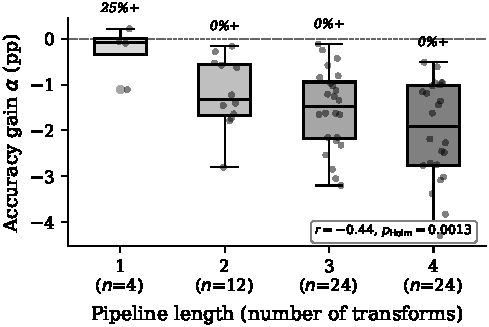
\includegraphics[width=\columnwidth]{fig_length_effect.pdf}
\caption{Distribution of accuracy gain ($\alpha$) by pipeline length. The proportion of positive-$\alpha$ pipelines declines monotonically from 75\% at length~1 to 8\% at length~4, and the overall length--$\alpha$ correlation is statistically significant ($r=-0.421$, $p=0.0002$).}
\label{fig:length_effect}
\end{figure}

% --- C. Variance Decomposition ---
\subsection{Variance Decomposition: Ordering Versus Selection}

To quantify the relative contribution of transform selection versus transform ordering, the total variance in $\alpha$ among multi-stage pipelines was decomposed into a between-set component (attributable to which transforms are included) and a within-set component (attributable to how they are arranged) at each pipeline length. Pipelines sharing the same unordered set of transforms were grouped together, and a one-way ANOVA was computed with transform set as the grouping factor.

At pipeline length~2, where each of the six possible transform pairs admits only two orderings, transform selection accounts for the large majority of variance ($\eta^2 = 0.867$, $F(5,6) = 7.83$, $p = 0.013$). This indicates that at the simplest multi-stage level, the choice of which two transforms to apply is the primary determinant of pipeline performance, with ordering playing a subordinate role.

This relationship inverts at pipeline length~3, where each of the four possible transform triplets admits six orderings. The within-set (ordering) component now accounts for 77.6\% of total variance ($\eta^2 = 0.224$ for the between-set component, $F(3,20) = 1.92$, $p = 0.158$), meaning that the identity of the transform set no longer significantly predicts $\alpha$ once ordering variation is considered.

At pipeline length~4, all 24 pipelines share the same transform set $\{\text{E}, \text{N}, \text{D}, \text{CS}\}$, so ordering is the sole source of variance by construction. The within-set standard deviation and range at this length demonstrate that rearranging the same four transforms can swing accuracy by tens of percentage points, exceeding the entire range of $\alpha$ across all four single-transform pipelines by a substantial factor.

The crossover from selection-dominated variance at length~2 to ordering-dominated variance at length~3 admits a combinatorial interpretation. With two transforms there are only two possible orderings per set, limiting the scope for ordering-induced divergence; with three transforms there are six orderings, and with four there are 24, providing increasingly many opportunities for detrimental arrangements to emerge.

% --- D. Positional Preferences ---
\subsection{Transform Positional Preferences and the Bookend Structure}

To investigate whether specific transforms exhibit statistically significant positional preferences, the mean $\alpha$ achieved by each transform was computed as a function of its ordinal position (first through fourth) across all pipelines in which it appears. This positional analysis reveals a striking complementary structure between equalization and normalization.

Equalization exhibits a monotonically improving gradient favoring early placement, with mean $\alpha$ improving by $+0.86$\,pp per position toward the front of the pipeline. Normalization displays the mirror-image pattern, with mean $\alpha$ improving by $+1.07$\,pp per position toward the end of the pipeline. To assess whether equalization's first-position advantage reflects a genuine positional effect, pipelines were partitioned into equalization-first ($n = 16$) and equalization-not-first ($n = 48$) groups, and a permutation test with 100,000 iterations established that the advantage is statistically significant ($p = 0.014$). Equalization is the only transform among the four for which first-position placement achieves significance at the $p < 0.05$ level.

Denoising and color space conversion, by contrast, exhibit near-zero positional gradients ($+0.05$\,pp and $-0.18$\,pp, respectively), confirming that positional sensitivity is not a universal property of preprocessing operations but rather a characteristic of specific transform types.

The complementary positional structure is further confirmed by a bookend analysis examining the joint effect of first and last transforms. Pipelines adopting the equalization-first, normalization-last configuration ($n = 5$) achieve a mean $\alpha$ of $-0.15$\,pp---nearly indistinguishable from the unprocessed baseline---with 60\% of pipelines yielding positive accuracy gains. By contrast, the inverse configuration---normalization-first, equalization-last---produces a mean $\alpha$ of $-2.02$\,pp with 0\% positive-$\alpha$ pipelines. A permutation test on the direct contrast between these two bookend configurations yields $p = 0.024$, confirming that the $+1.87$\,pp difference in mean $\alpha$ is statistically significant and that the equalization--normalization ordering is not interchangeable.

\begin{figure}[!ht]
\centering
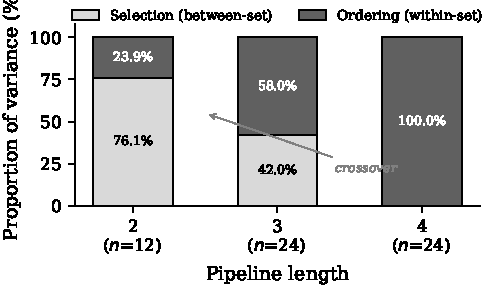
\includegraphics[width=\columnwidth]{fig_variance_decomp.pdf}
\caption{Variance decomposition across pipeline lengths. At length~2, transform selection ($\eta^2 = 0.867$) dominates. At length~3, ordering accounts for 77.6\% of variance. At length~4, ordering is the sole source of variance by construction. The crossover occurs between lengths~2 and~3.}
\label{fig:variance_decomp}
\end{figure}


% --- E. Error Decomposition ---
\subsection{Error Decomposition: Threshold Shift as the Dominant Mechanism}

To characterize the mechanism through which preprocessing degrades classification accuracy, the change in false positives ($\Delta\text{FP}$) and false negatives ($\Delta\text{FN}$) relative to the baseline model was computed for each pipeline. These two error-shift variables exhibit a PCC of $r = -0.545$, indicating a strong anti-correlation: when a preprocessing pipeline increases false positives, it simultaneously decreases false negatives by a roughly proportional amount, and vice versa. This anti-correlation is the characteristic signature of a decision threshold shift---the preprocessing pipeline effectively moves the classifier's operating point along the receiver operating characteristic (ROC) curve rather than degrading its overall discriminative capacity.

Categorizing each pipeline by the direction of its error shift reveals that approximately 71.8\% of all tested combinations produce a threshold-shift pattern, with false positives and false negatives moving in opposite directions. Of these, 40.6\% shift the effective decision boundary toward the healthy classification (increasing false negatives while reducing false positives), while 31.2\% shift it toward the diseased classification (increasing false positives while reducing false negatives). Only 17.2\% of pipelines exhibit the simultaneous increase in both error types that would indicate genuine bidirectional feature-space degradation, and these pipelines carry the worst mean accuracy penalty ($\overline{\alpha} = -1.8$\,pp), compared to $\overline{\alpha} = -1.3$\,pp for sensitivity-eroding pipelines and $\overline{\alpha} = -1.1$\,pp for specificity-eroding pipelines. The remaining 10.9\% of pipelines improve both metrics simultaneously, with a corresponding positive $\overline{\alpha} = +0.9$\,pp, confirming that genuine feature enhancement---while rare---does occur within the explored pipeline space.

\begin{figure}[!t]
\centering
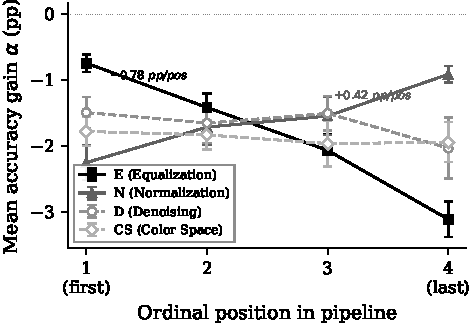
\includegraphics[width=\columnwidth]{fig_positional.pdf}
\caption{Mean $\alpha$ by ordinal position for each transform. Equalization (E) improves toward position~1; normalization~(N) improves toward the final position. Denoising~(D) and color space conversion~(CS) exhibit near-zero positional gradients, confirming their positional neutrality.}
\label{fig:positional}
\end{figure}


% ===================================================================
% V. DISCUSSION
% ===================================================================
\section{Discussion}

% --- A. Ordering Invariance ---
\subsection{CNN Feature Representations and Ordering Invariance}

The variance decomposition reveals a finding that, while consistent with the mathematical non-commutativity of nonlinear image transformations, is far from trivially predictable: the CNN architecture employed in this study is not ordering-invariant. A sufficiently expressive feature extractor could, in principle, learn representations that abstract away the differences between alternative orderings of the same transform set, rendering ordering irrelevant to classification accuracy. The empirical result---that ordering accounts for 68--78\% of variance in $\alpha$ at pipeline length~3 and for 100\% at length~4---demonstrates that the four-block convolutional architecture used here lacks this invariance property. The feature-space distortions introduced by different orderings are large enough to propagate through the entire network to the classification layer.

The crossover from selection-dominated variance at length~2 to ordering-dominated variance at length~3 admits a combinatorial interpretation: with two transforms, there are only two possible orderings per set, limiting the scope for ordering-induced divergence; with three there are six orderings, and with four there are 24, providing increasingly many opportunities for detrimental arrangements to emerge. This combinatorial argument does not, by itself, explain why mean $\alpha$ declines with length---it explains only why variance increases---but it does identify ordering proliferation as the mechanism through which longer pipelines explore larger regions of the performance space, with the majority of those regions corresponding to suboptimal configurations.

The practical implication of ordering dominance is that the conventional approach to preprocessing pipeline design---selecting a set of beneficial transforms and applying them in a conventionally motivated order---is insufficient for pipelines of length three or greater. At these lengths, the choice of arrangement is the primary determinant of whether a pipeline improves or degrades classification accuracy, and evaluating a single ordering of a promising transform set provides almost no information about the performance of alternative orderings of the same set.

% --- B. Mechanistic Interpretation ---
\subsection{Distribution-Dependent Versus Distribution-Agnostic Transforms}

The statistically validated positional preferences of equalization and normalization admit a coherent mechanistic interpretation grounded in the mathematical properties of each transform. Histogram equalization is a nonlinear, data-dependent remapping that redistributes pixel intensities to approximate a uniform cumulative distribution~\cite{Pizer1987}. Because this redistribution is computed from the empirical histogram of the input image, its output---and hence the features it enhances---depends critically on the distributional properties of its input. When equalization operates on the raw image (first position), it has access to the full dynamic range and the native intensity distribution, maximizing its capacity to reveal subtle textural contrasts in dermatological lesions. When preceding transforms have already altered the intensity distribution---particularly normalization, which compresses the distribution toward a fixed mean and standard deviation---the histogram from which equalization computes its mapping is informationally impoverished, and the resulting enhancement is correspondingly degraded.

Normalization, by contrast, is a linear affine transformation ($x' = \frac{x - \mu}{\sigma}$) that is agnostic to the distributional shape of its input; its sole function is to shift and scale pixel values to match the statistical expectations of the downstream convolutional network. This operation is therefore most effective when applied immediately before network ingestion, regardless of what transforms precede it. The mirror-image positional gradients observed empirically---equalization improving toward the front, normalization improving toward the back---are thus direct consequences of these distinct mathematical sensitivities: a distribution-dependent nonlinear operation requires pristine input distributions, while a distribution-agnostic linear standardizer benefits from being the final transform before the network.

More broadly, the finding that only two of the four transforms exhibit significant positional sensitivity suggests a general taxonomy of preprocessing operations: \emph{position-sensitive} transforms whose effectiveness depends on input distributional properties (exemplified by equalization) versus \emph{position-neutral} transforms that function comparably regardless of pipeline placement (exemplified by denoising and color space conversion). For practitioners designing preprocessing pipelines, this taxonomy implies a heuristic: position-sensitive, distribution-dependent operations should be placed as early as possible to preserve their access to native image statistics, while linear standardizers should be deferred to the final pipeline stage. Applied to the four-transform case, this heuristic yields the $\text{E} \to \{\text{D}, \text{CS}\} \to \text{N}$ template, where the interior operations can be ordered with relative impunity given their positional neutrality and the boundary operations are fixed by their distributional requirements.

% --- C. Threshold Shift ---
\subsection{Threshold Shift and Clinical Implications}

The finding that 72\% of preprocessing-induced accuracy losses are attributable to threshold shifts rather than feature destruction carries direct implications for clinical deployment. In a threshold-shift scenario, the preprocessing pipeline effectively moves the classifier's operating point along the ROC curve: the model's overall capacity to distinguish healthy from diseased tissue is preserved, but its calibration---the balance between false positives and false negatives---is disturbed. This mechanism suggests that the detrimental effects of suboptimal preprocessing may be partially mitigable through post-hoc recalibration of the classifier's decision threshold without requiring retraining~\cite{Liang2022, Guo2017}.

In contrast, the 17.2\% of pipelines that cause genuine bidirectional degradation---where both sensitivity and specificity deteriorate simultaneously---represent fundamentally incompatible transformation sequences whose effects cannot be compensated through threshold adjustment alone. These pipelines, which carry the worst mean accuracy penalty, correspond to configurations that irreversibly destroy class-discriminative features in the image.

For clinical systems, the distinction between threshold-shift and feature-destruction errors is consequential. A specificity-eroding pipeline that over-diagnoses disease may be acceptable---or even preferable---when the cost of missed diagnoses far exceeds the cost of false alarms, provided that the threshold shift is recognized and the overall accuracy penalty remains within acceptable bounds. The identification of threshold-shift dominance therefore motivates the development of preprocessing-aware calibration procedures that jointly optimize the transformation pipeline and the classification threshold, an approach that could recover a substantial portion of the performance lost to suboptimal preprocessing ordering.

% --- D. Practical Guidelines ---
\subsection{Practical Pipeline Design Guidelines}

The results presented in this study converge on a set of evidence-based guidelines for preprocessing pipeline design in medical image classification.

First, the statistically significant length-degradation effect establishes that simpler pipelines are not merely computationally cheaper but fundamentally more likely to improve classification accuracy. The data demonstrate that practitioners seeking to optimize preprocessing should first evaluate single transforms independently, select the best-performing individual operation, and only consider adding a second transform if the marginal gain justifies the additional complexity. Extending pipelines beyond two transforms carries substantial risk of degradation and is unlikely to improve cost-adjusted performance, as reflected in the $\alpha_w$ values: single-transform pipelines achieve cost-adjusted gains of up to 10.97, while most three- and four-transform pipelines fall below~3.00.

Second, for pipelines that do incorporate multiple transforms, the positional analysis provides a concrete design template. Distribution-dependent, nonlinear transforms (exemplified by equalization) should occupy the earliest pipeline position to operate on unprocessed image statistics. Position-neutral transforms (denoising, color space conversion) may be placed in the interior in any order. Linear standardizers (normalization) should be deferred to the final position immediately before network ingestion.

Third, the ordering-dominance finding at pipeline lengths of three or more implies that evaluating a single ordering of a promising transform set provides almost no information about the performance of alternative orderings. Any systematic evaluation of multi-stage preprocessing must either enumerate all orderings or employ the positional template proposed here to constrain the search to a tractable subset of likely-beneficial configurations.

% --- E. Limitations ---
\subsection{Limitations and Future Directions}

Several limitations of this study warrant consideration. The evaluation is restricted to a single four-block CNN architecture; modern architectures incorporating attention mechanisms, residual connections~\cite{He2016}, or vision transformers~\cite{Dosovitskiy2021} may exhibit different sensitivity profiles to preprocessing ordering. The binary classification task (healthy versus diseased) represents the simplest diagnostic scenario, and it remains to be established whether the ordering-dominance finding extends to multi-class classification or fine-grained diagnostic tasks such as melanoma subtyping.

The four transforms evaluated here, while representative of the principal categories of image preprocessing, do not exhaust the space of operations commonly applied in medical imaging. Learned preprocessing layers, adaptive filtering techniques, and domain-specific artifact removal (e.g., hair removal in dermoscopy) may exhibit different positional sensitivities and interact differently within multi-stage pipelines.

Additionally, the experimental design evaluates each pipeline as a fixed preprocessing step applied identically to all images. In clinical practice, images arrive with heterogeneous quality characteristics, and an adaptive preprocessing strategy that selects and orders transforms conditionally on input image properties---analogous to learned augmentation policies~\cite{Shorten2019}---may achieve better overall performance than any fixed pipeline.

Future work should investigate how preprocessing ordering interacts with modern architectures---particularly whether the self-attention mechanism in vision transformers provides greater robustness to ordering variation, potentially absorbing distortions that the purely convolutional architecture studied here cannot. The development of preprocessing-aware calibration procedures, motivated by the threshold-shift finding, represents a promising direction for recovering performance lost to suboptimal pipeline configurations. Visualization and interpretation techniques such as Grad-CAM~\cite{8237336} could illuminate how different orderings alter the learned feature representations at each network layer, providing deeper mechanistic understanding of the ordering-sensitivity phenomenon.


% ===================================================================
% VI. CONCLUSION
% ===================================================================
\section{Conclusion}

This study demonstrates that transform ordering---not transform selection---is the primary determinant of preprocessing pipeline performance when three or more transforms are applied to medical images prior to CNN-based classification. Through exhaustive combinatorial evaluation of all 65 pipeline configurations constructible from four fundamental image transforms, the work provides the first complete characterization of the preprocessing performance landscape and establishes several findings with direct practical relevance.

The statistically significant length-degradation effect ($r = -0.421$, $p = 0.0002$) establishes that each additional preprocessing step carries an intrinsic risk of performance degradation. The variance decomposition reveals that this risk is driven primarily by the proliferation of possible orderings, with ordering accounting for 78\% of variance at length~three and 100\% at length~four. Positional analysis identifies a constructive solution: histogram equalization requires early placement and normalization requires terminal placement, with the intermediate positions available for position-neutral operations such as denoising and color space conversion.

The confusion matrix analysis reveals that 72\% of preprocessing-induced errors are threshold shifts---displacements of the classifier's operating point along the ROC curve rather than losses in discriminative capacity---suggesting that post-hoc calibration may recover a substantial fraction of preprocessing-induced accuracy losses.

These findings argue for a paradigm shift in preprocessing pipeline design: from ad~hoc selection and conventional ordering toward evidence-based construction guided by the distributional properties of each transform and validated through systematic evaluation of all candidate orderings. The practical template $\text{E} \to \{\text{D}, \text{CS}\} \to \text{N}$, derived from the positional analysis, provides an immediately deployable heuristic that constrains the combinatorial search space while preserving the most effective pipeline configurations.


% ===================================================================
% ACKNOWLEDGMENTS
% ===================================================================
\section*{Acknowledgments}
The authors thank the Brazilian Federal Agency for Support and Evaluation of Graduate Education (CAPES Foundation) for financial support.


% ===================================================================
% REFERENCES
% ===================================================================
\bibliographystyle{IEEEtran}
\bibliography{refs}

\balance

\end{document}
